\documentclass{article}
\usepackage{graphicx}
\graphicspath{ {images/} }
\usepackage{hyperref}
\usepackage[margin=0.5in]{geometry}

\begin{document}

\section*{Show Facebook Calendars on SFU Website}

\begin{enumerate}
	\item \textbf{Getting facebook calendar subscription Link}
	\begin{itemize}
		\item log in with "thomasaanderson" account
		\item Click on Events
		
		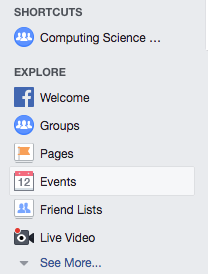
\includegraphics[scale=0.45]{picture1.png}
		\item Right click on "Upcoming Events" and select "Save Link As"
		
		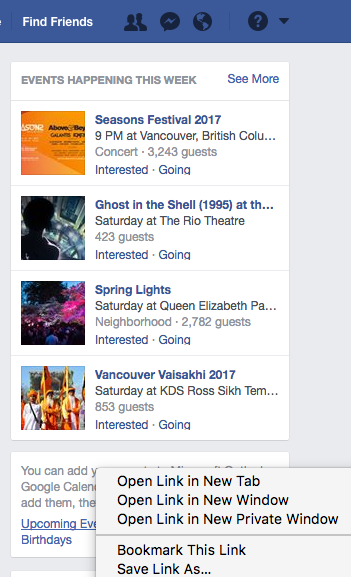
\includegraphics[scale=0.45]{picture2.png}
		\item the above steps give you this link: 
		
		\url{http//www.facebook.com/ical/u.php?uid=100016344735432&key=AQBVgDJ7N5vql8sp}
	\end{itemize}
	\item \textbf{Adding subscription link to google calendar account}
	\begin{itemize}
		\item go to calendar page for sfucsss gmail account
		\item click on right down arrow next to "other calendar" and choose "Add by URL"
		
		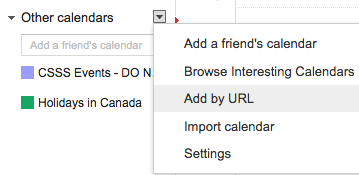
\includegraphics[scale=0.45]{picture3.png}
		\item enter in the subscription link obtained into the URL and make sure to make the calendar publicly accessible
	\end{itemize}
	\item \textbf{Share google calendar to sfucsss website}
	\begin{itemize}
		\item click on arrow next to recently added calendar in "other calendar"
		
		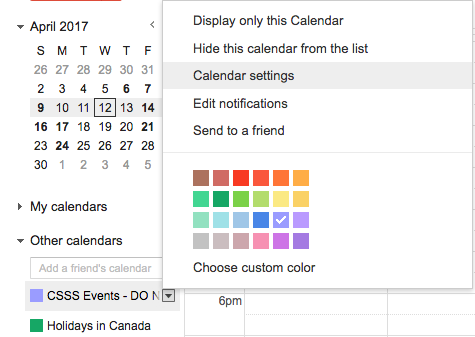
\includegraphics[scale=0.45]{picture4.png}
		\item select "calendar settings"
		\item click on "Customize the color, size, and other options" in the attached picture
		
		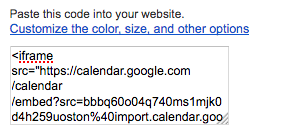
\includegraphics[scale=0.45]{picture5.png}
		\item Enter a space in the "Calender Title" field to hide the "CSSS Events - DO NOT UNSUBSCRIBE" title from the calendar
		\item Also unclick "Calendar list" in the left checkboxes
		\item Ensure in "Calendars to display" in the bottom left side of page, only "Thomas Anderson's Facebook Events" is selected
		\item Click "Update HTML" button next to "Copy and paste the HTML below to include this calendar on your webpage"
		\item copy the generated HTML code and paste it into the sfucss upcoming events post contents editor
	\end{itemize}
\end{enumerate}

		
\end{document}